\chapter{Virologi}\label{ch:b3:virology}

Terdapat sekitar $10^{31}$ partikel \omterm{def:b3:virology:virus}{virus} di Bumi, sepuluh bagi tiap sel,
dan di laut mereka membunuh seperlima seluruh bakteri setiap hari. Sebuah \omterm{def:b3:virology:virus}{virus}
bukanlah sel: ia tidak bermetabolisme, tidak berribosom, dan tidak punya cara
membuat apa pun sendiri. Ia adalah sebuah genom --- sependek dua gen, sepanjang
dua ribu --- yang terbungkus cangkang protein, yang memasuki sebuah sel lalu
mengubah mesin sel itu menjadi pembuat salinan dirinya. Influenza tahun 1918
membunuh lima puluh juta orang; cacar, yang membunuh tiga ratus juta orang pada
abad kedua puluh saja, dibasmi pada tahun 1980 oleh sebuah \omterm{def:b3:virology:drugs}{vaksin} yang pertama
kali dicoba pada tahun 1796; dan sebuah koronavirus yang menyeberang ke manusia
pada tahun 2019 genomnya terurutkan dalam hitungan minggu, sebuah \omterm{def:b3:virology:drugs}{vaksin}
dirancang dalam hitungan hari sesudahnya, dan obat terhadap proteasenya dalam
dua tahun. Bab ini memperlakukan apa itu \omterm{def:b3:virology:virus}{virus} dan bagaimana ia digolongkan
menurut kimia genomnya, bagaimana ia memperbanyak diri, kinetika sebuah infeksi
di dalam satu inang --- yang digambarkan sepasang persamaan diferensial cukup
baik hingga mengubah pengobatan AIDS --- evolusinya, serta bagaimana ia dilawan.

\section{Apa itu virus}

\begin{definition}[Virus]\label{def:b3:virology:virus}
\index{virus}\index{kapsid}\index{selubung}%
\index{virion}\index{klasifikasi Baltimore}
Sebuah \emph{virus} adalah parasit intrasel obligat yang terdiri atas sebuah
genom asam nukleat --- DNA atau RNA, untai tunggal atau untai ganda, lurus
atau melingkar, satu molekul atau beberapa --- yang terkemas di dalam sebuah
\emph{kapsid} protein, dan dalam banyak hal terbungkus sebuah \emph{selubung}
yang diambil dari membran inang serta bertaburan glikoprotein virus. Partikel
menular yang lengkap adalah \emph{virion}, yang bagi kebanyakannya berukuran
\qtyrange{20}{300}{nm} (beberapa virus raksasa mencapai satu mikrometer).
Kapsid dibangun dari banyak salinan satu atau beberapa protein yang tersusun
dengan simetri heliks (sebuah batang, seperti pada virus mosaik tembakau) atau
simetri ikosahedral (sebuah cangkang beranggota $60T$ subunit, dengan
$T = 1, 3, 4, 7,\dots$). \emph{Klasifikasi Baltimore} menggolongkan virus
menurut jalan dari genom ke RNA duta: I, DNA untai ganda (herpes, cacar,
adenovirus, sebagian besar fag); II, DNA untai tunggal (parvovirus); III, RNA
untai ganda (rotavirus); IV, RNA untai positif, yang dirinya sendiri sebuah
duta (polio, hepatitis C, koronavirus); V, RNA untai negatif, yang komplemen
terhadap duta (influenza, campak, rabies, Ebola); VI, RNA yang ditranskripsi
balik menjadi DNA (retrovirus, HIV); VII, DNA yang digandakan lewat sebuah
antara RNA (hepatitis B). Setiap kelas selain I harus membawa atau menyandi
sebuah enzim yang tidak dipunyai sel --- sebuah RNA polimerase bergantung-RNA,
sebuah transkriptase balik --- dan enzim itulah sasaran kebanyakan \omterm{def:b3:virology:drugs}{obat
antivirus}.
\end{definition}

\begin{proof}[Bukti eksperimental]
Ivanovsky (1892) dan Beijerinck (1898) menunjukkan bahwa penyakit mosaik pada
tembakau ditularkan oleh getah yang dilewatkan melalui saringan yang menahan
seluruh bakteri --- sebuah \emph{contagium vivum fluidum}, yakni cairan hidup
yang menular. Stanley (1935) menghablurkan agennya, yakni \omterm{def:b3:virology:virus}{virus} mosaik
tembakau, lalu menunjukkan bahwa agen itu berupa protein dengan (sebagaimana
ditemukan Bawden dan Pirie) \qty{5}{\%} RNA. Hershey dan Chase (1952) menandai
protein sebuah bakteriofag dengan $^{35}$S dan DNA-nya dengan $^{32}$P,
membiarkannya menginfeksi \emph{E.~coli}, menggunting lepas mantel kosongnya
di dalam sebuah pengaduk, lalu menemukan $^{32}$P di dalam selnya dan $^{35}$S
di luarnya: DNA-lah yang masuk dan proteinnya tertinggal, sehingga DNA itulah
pembawa petunjuknya. Fraenkel-Conrat (1955) mengurai \omterm{def:b3:virology:virus}{virus} mosaik tembakau
menjadi protein dan RNA lalu menyusun kembali partikel menular dari RNA satu
galur dan protein galur lain; keturunannya bergalur seperti RNA-nya.
\end{proof}

\begin{proposition}[Ekonomi genetik: mengapa kapsid bersimetri]\label{prop:b3:virology:economy}
\index{ekonomi genetik}
Sebuah \omterm{def:b3:virology:virus}{kapsid} harus mengurung genom yang menyandinya. Sebuah protein bermassa
$m$ memerlukan sekitar $m/\qty{110}{Da}$ kodon, yakni $3m/110$ nukleotida,
yaitu sepotong RNA yang berbobot sekitar $3m/110\times\qty{330}{Da} = 9m$: tiap
protein disandi oleh asam nukleat yang bermassa sembilan kali massanya sendiri.
Sebuah cangkang yang dibuat dari \emph{satu} molekul protein yang mengurung
sebuah genom harus mengurung genom bermassa sembilan kali massanya sendiri
hanya untuk menyandi dirinya, padahal sebuah cangkang tidak dapat memuat asam
nukleat sembilan kali massanya sendiri pada kerapatan biologis. Jalan
keluarnya, yang dilihat Crick dan Watson (1956), adalah membangun cangkang itu
dari banyak salinan satu protein kecil: \omterm{def:b3:virology:virus}{virus} mosaik tembakau menyandi sebuah
protein mantel \qty{17.5}{kDa} di dalam \qty{480}{nt} dari genomnya yang
\qty{6400}{nt}, lalu memakai $2130$ salinannya. Subunit yang serupa dan
berkemas serupa harus tersusun secara simetris, sehingga \omterm{def:b3:virology:virus}{kapsid} \omterm{def:b3:virology:virus}{virus} berupa
heliks atau ikosahedron, dan ekonomi yang sama memberinya kemampuan merakit
diri, sebab tiap subunit hanya perlu mengenali tetangganya.
\end{proposition}
\begin{proof}
Nisbah massanya menyusul dari sebuah kodon yang berupa tiga nukleotida yang
masing-masing sekitar \qty{330}{Da} dan sebuah residu yang sekitar
\qty{110}{Da}: $3\times 330/110 =
9$. Sebuah \omterm{def:b3:virology:virus}{kapsid} dari satu protein \qty{40}{MDa} akan mengurung
\qty{360}{MDa} asam nukleat, yakni sebuah bola berjejari sekitar \qty{50}{nm}
pada kerapatan asam nukleat, sedangkan proteinnya sendiri akan membuat sebuah
cangkang setebal sekitar \qty{2}{nm} dengan jejari yang sama --- mungkin secara
geometris, tetapi sebuah polipeptida tunggal beranggota $360\,000$ residu yang
melipat dengan benar tidaklah mungkin, dan satu mutasi akan merusaknya. Dengan
$n$ subunit yang serupa, ongkos penyandiannya turun sebesar $n$ sementara
volume yang terkurung tidak berubah.
\end{proof}

\begin{omfigure}
\begin{tikzpicture}[every node/.style={font=\scriptsize}, >=stealth]
  \node[draw, thick, rounded corners, fill=omMeth!30, minimum width=2.4cm] (mrna) at (0,0) {RNA duta $\to$ protein};
  \node[draw, thick, rounded corners, fill=omDef!20, align=center] (I) at (-5.8,3.6) {I: DNA untai ganda\\herpes, cacar, fag T4};
  \node[draw, thick, rounded corners, fill=omDef!20, align=center] (II) at (-2.0,3.6) {II: DNA untai tunggal\\parvovirus};
  \node[draw, thick, rounded corners, fill=omThm!20, align=center] (III) at (2.0,3.6) {III: RNA untai ganda\\rotavirus};
  \node[draw, thick, rounded corners, fill=omThm!20, align=center] (IV) at (5.8,3.6) {IV: RNA (+)\\polio, hepatitis C,\\koronavirus};
  \node[draw, thick, rounded corners, fill=omThm!20, align=center] (V) at (-5.6,-3.4) {V: RNA ($-$)\\influenza, campak,\\rabies, Ebola};
  \node[draw, thick, rounded corners, fill=omProp!30, align=center] (VI) at (0,-3.4) {VI: RNA $\to$ DNA\\retrovirus (HIV)};
  \node[draw, thick, rounded corners, fill=omProp!30, align=center] (VII) at (5.6,-3.4) {VII: DNA lewat RNA\\hepatitis B};
  \node[below, font=\tiny, align=center, gray!50!black] at (-5.8,2.9) {RNA polimerase inang};
  \node[below, font=\tiny, align=center, gray!50!black] at (-2.0,3.05) {untai kedua dibuat,\\lalu transkripsi};
  \node[below, font=\tiny, align=center, gray!50!black] at (2.0,3.05) {RNA polimerase virus\\di dalam partikelnya};
  \node[below, font=\tiny, align=center, gray!50!black] at (5.8,2.75) {genomnya adalah mRNA};
  \node[above, font=\tiny, align=center, gray!50!black] at (-5.6,-2.55) {polimerase virus menyalinnya};
  \node[above, font=\tiny, align=center, gray!50!black] at (0,-2.85) {transkriptase balik, penyisipan,\\lalu polimerase inang};
  \node[above, font=\tiny, align=center, gray!50!black] at (5.6,-2.85) {transkripsi DNA-nya};
  \foreach \c in {I,II,III,IV,V,VI,VII} \draw[->, thick] (\c) -- (mrna);
\end{tikzpicture}

{\small Tujuh kelas Baltimore, yang tersusun menurut jalan dari genom ke RNA
duta. Setiap kelas selain I memerlukan sebuah enzim yang tidak disediakan sel
inang --- sasaran alami sebuah \omterm{def:b3:virology:drugs}{obat antivirus}.}
\end{omfigure}

\begin{omfigure}
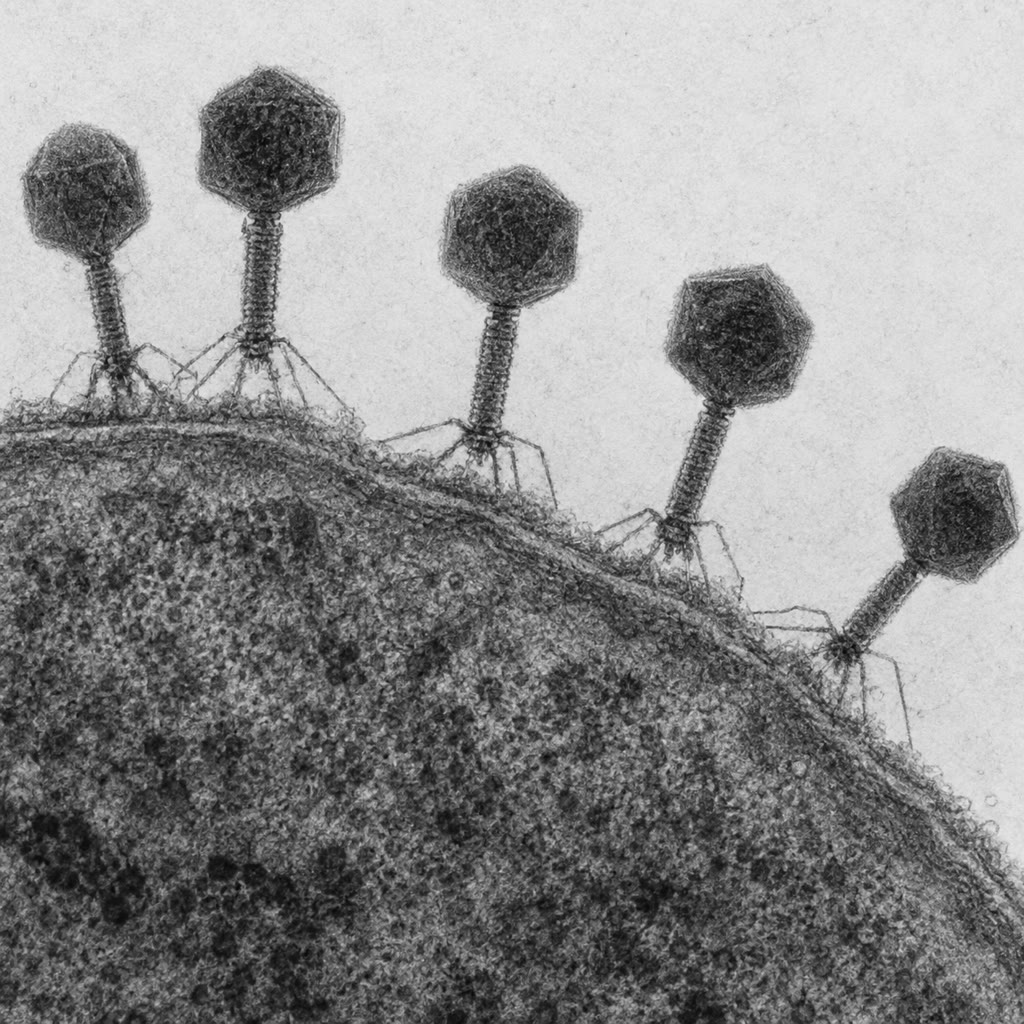
\includegraphics[width=0.36\linewidth]{images/book5/ai/b5-13-phage-tem.jpg}\hspace{0.04\linewidth}
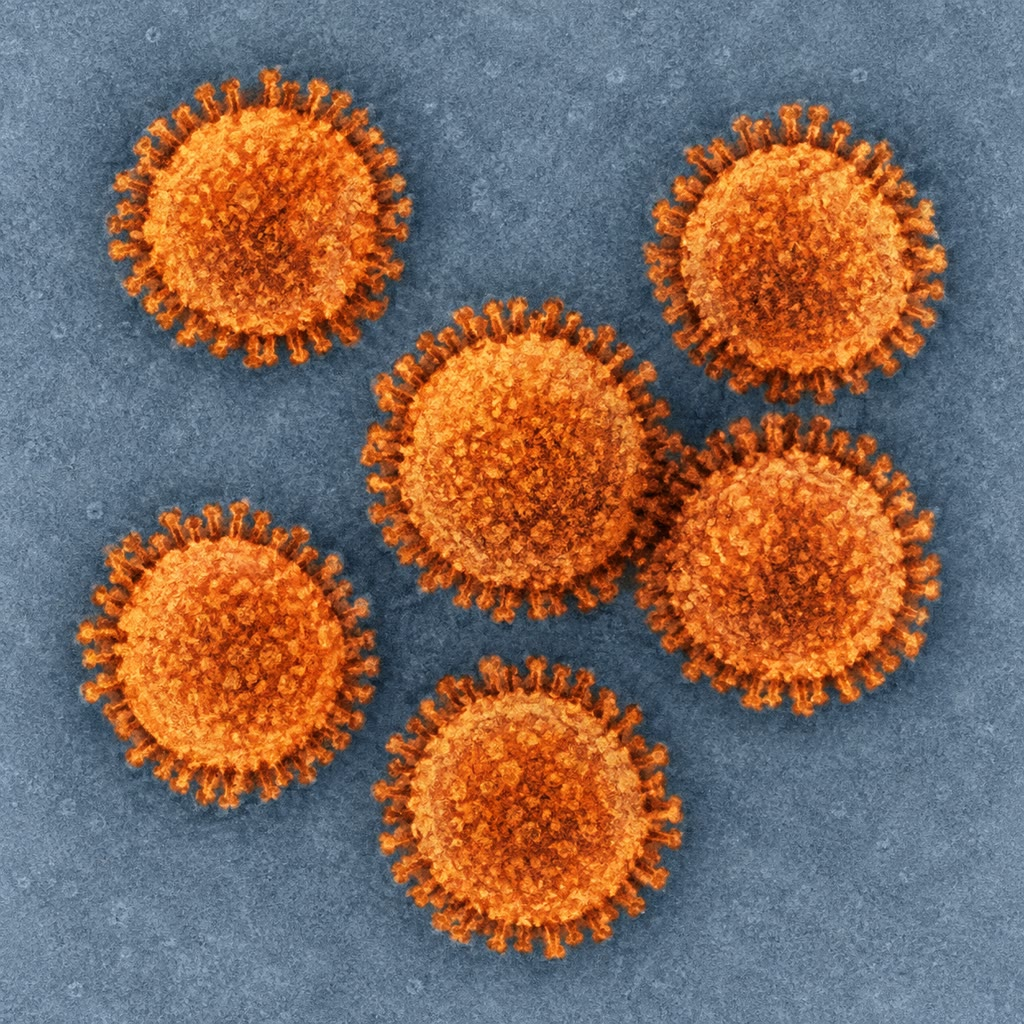
\includegraphics[width=0.36\linewidth]{images/book5/ai/b5-13-influenza-virions.jpg}

{\small Kiri: bakteriofag yang melekat lewat serat ekornya pada sebuah
bakteri, tiap kepalanya sebuah \omterm{def:b3:virology:virus}{kapsid} ikosahedral berisi DNA. Kanan: \omterm{def:b3:virology:virus}{virion}
influenza, yang berselubung, dengan permukaan berupa rumbai duri hemaglutinin
dan neuraminidase.}
\end{omfigure}

\section{Bagaimana virus memperbanyak diri}

\begin{definition}[Daur replikasi]\label{def:b3:virology:cycle}
\index{daur replikasi virus}\index{reseptor!virus}%
\index{lisogeni}\index{latensi}
Setiap \omterm{def:b3:virology:virus}{virus} melewati tahap yang sama. \emph{Pelekatan} pada sebuah reseptor
inang tertentu --- CD4 dan sebuah reseptor kemokin bagi HIV, ACE2 bagi
koronavirus SARS, asam sialat bagi influenza, sebuah \omterm{def:b3:bacteriology:envelope}{lipopolisakarida} atau
sebuah porin bagi sebuah fag --- yang memutuskan spesies dan sel mana yang
dapat diinfeksi \omterm{def:b3:virology:virus}{virus} itu (yakni \emph{tropisme}-nya).
\emph{Pemasukan}: peleburan \omterm{def:b3:virology:virus}{selubung} \omterm{def:b3:virology:virus}{virus} dengan membran plasma, atau
endositosis yang disusul peleburan dari dalam \omterm{def:b3:membrane-traffic:endocytosis}{endosom} yang asam, atau, bagi
sebuah fag, penyuntikan genom menembus dindingnya. \emph{Pengupasan mantel},
\emph{pengungkapan} gen \omterm{def:b3:virology:virus}{virus} lewat jalan yang khas bagi kelasnya, serta
\emph{replikasi} genomnya, kerap di dalam sebuah pabrik yang dibangun \omterm{def:b3:virology:virus}{virus} itu
di dalam sitoplasma atau inti. \emph{Perakitan} \omterm{def:b3:virology:virus}{kapsid} baru di sekeliling genom
baru, yang didorong oleh perakitan diri subunit yang simetris, lalu
\emph{pelepasan}: dengan melisiskan selnya, atau dengan menguncup menembus
sebuah membran, yang memasok \omterm{def:b3:virology:virus}{selubungnya}. Sebagian \omterm{def:b3:virology:virus}{virus} dapat justru
menyisipkan genomnya ke dalam genom inang lalu menunggu: \emph{lisogeni} fag
$\lambda$, yang penekannya menjaganya tetap bungkam sampai inangnya rusak;
\emph{latensi} herpesvirus di dalam neuron seumur hidup dan latensi HIV sebagai
sebuah provirus di dalam sel~T yang beristirahat, yang darinya ia tidak
disingkirkan oleh obat apa pun yang bekerja pada replikasi.
\end{definition}

\begin{omfigure}
\begin{tikzpicture}[every node/.style={font=\scriptsize}, >=stealth]
  % cell
  \draw[very thick, omDef, fill=omDef!6] (0,0) ellipse (5.6 and 3.2);
  \draw[thick, omDef!70, fill=omDef!20] (1.8,0) ellipse (1.6 and 1.1); \node at (1.8,0.75) {inti};
  % virion outside
  \draw[thick, omProp, fill=omProp!30] (-7.2,1.6) circle (0.35); \foreach \a in {0,45,...,315} \draw[omProp, thick] (-7.2,1.6) ++(\a:0.35) -- ++(\a:0.15);
  \node[above] at (-7.2,2.1) {virion};
  \draw[->, thick] (-6.8,1.4) -- (-5.7,0.9); \node[below, align=center] at (-6.6,1.0) {1. melekat pada\\reseptor};
  % entry
  \draw[thick, omProp] (-5.4,0.7) arc[start angle=140, end angle=40, radius=0.5];
  \node[below, align=center] at (-3.9,-0.2) {2. melebur atau endositosis;\\3. mengupas mantel};
  % genome path
  \draw[omThm, very thick] (-3.4,0.2) .. controls (-2.6,0.6) .. (-1.8,0.4);
  \draw[->, thick] (-1.6,0.4) -- (-0.4,0.4);
  \node[above, align=center] at (-1.0,0.55) {4. mengungkapkan gen,\\menggandakan genom};
  \draw[omThm, very thick] (-1.0,-0.5) -- (0.4,-0.5); \draw[omThm, very thick] (-1.0,-0.75) -- (0.4,-0.75); \draw[omThm, very thick] (-1.0,-1.0) -- (0.4,-1.0);
  % assembly
  \foreach \p in {(1.2,-1.6),(1.9,-1.9),(2.6,-1.5)} { \draw[thick, omProp, fill=omProp!30] \p circle (0.25); }
  \node[below, align=center] at (1.9,-2.2) {5. merakit kapsid\\di sekeliling genom};
  % budding
  \draw[thick, omProp, fill=omProp!30] (4.9,-1.7) circle (0.32); \draw[->, thick] (5.3,-1.75) -- (6.4,-2.0);
  \draw[thick, omProp, fill=omProp!30] (7.0,-2.2) circle (0.35); \foreach \a in {0,45,...,315} \draw[omProp, thick] (7.0,-2.2) ++(\a:0.35) -- ++(\a:0.15);
  \node[below, align=center] at (6.4,-2.6) {6. menguncup lewat membran\\(selubung) atau melisiskan sel};
  % latency
  \draw[->, thick, dashed, omMeth!70!black] (-0.2,0.2) -- (0.9,0.2); \node[below, omMeth!70!black, align=center, font=\tiny] at (2.0,-0.05) {retrovirus: menyisip\\sebagai provirus; latensi};
\end{tikzpicture}

{\small Daur replikasi sebuah \omterm{def:b3:virology:virus}{virus} berselubung: pelekatan pada sebuah
reseptor, pemasukan dan pengupasan mantel, pengungkapan dan penggandaan di
dalam mesin inang, perakitan, lalu pelepasan dengan menguncup --- atau, bagi
sebuah retrovirus, penyisipan ke dalam genom inang lalu kebungkaman.}
\end{omfigure}

\begin{method}[Mencacah partikel menular: uji plak]\label{met:b3:virology:plaque}
\index{uji plak}\index{titer}
Untuk mengukur sebuah stok \omterm{def:b3:virology:virus}{virus}: (1) encerkanlah ia dalam langkah sepuluh kali
lipat; (2) campurkanlah tiap pengenceran dengan sel inang berlebih --- bakteri
di dalam agar lunak bagi sebuah fag, sebuah lapisan tunggal sel biakan bagi
sebuah \omterm{def:b3:virology:virus}{virus} hewan; (3) eramkanlah: tiap partikel menular menginfeksi satu sel,
keturunannya menginfeksi tetangganya, dan sesudah sehari atau dua hari sebuah
lubang bening, sebuah \emph{plak}, menandai tempatnya; (4) cacahlah plak pada
lempeng yang bermuatan \numrange{30}{300} lalu kalikanlah dengan pengencerannya:
itulah \emph{titer} dalam satuan pembentuk plak (PFU) per mililiter. Karena tiap
plak adalah klona satu partikel, memungutnya menghasilkan sebuah isolat murni.
Nisbah partikel fisis (yang dicacah dengan mikroskop elektron atau PCR) terhadap
satuan pembentuk plak biasanya jauh di atas satu --- sepuluh sampai seribu bagi
banyak \omterm{def:b3:virology:virus}{virus} hewan --- sebab kebanyakan partikel cacat atau gagal menginfeksi.
\end{method}

\begin{omfigure}
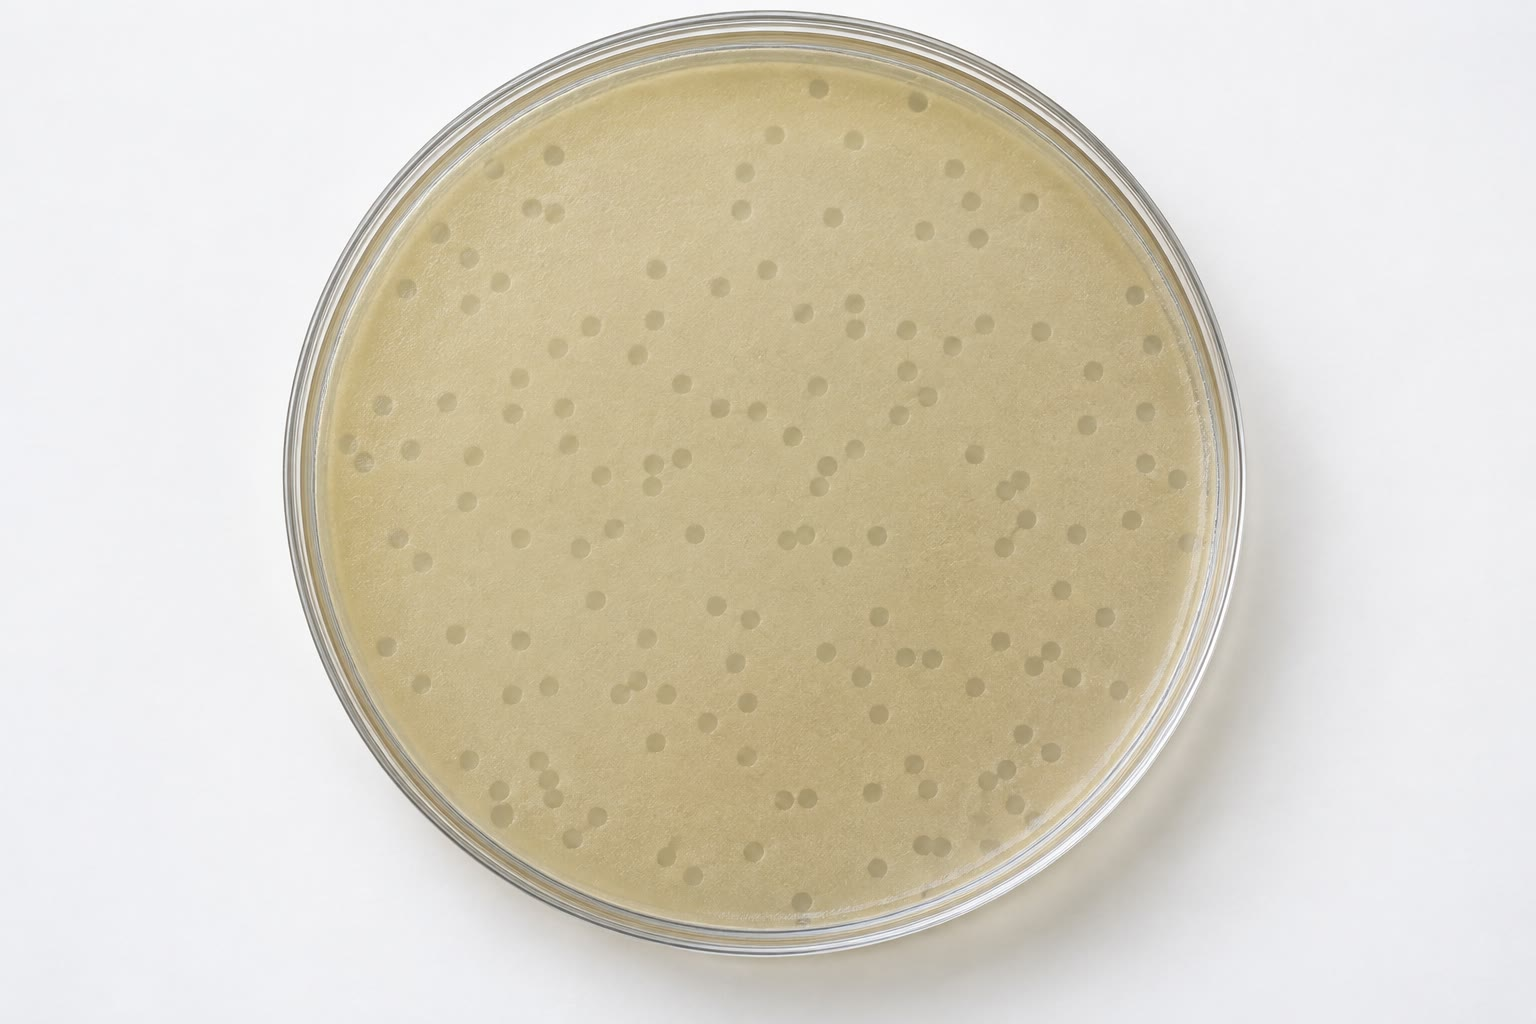
\includegraphics[width=0.46\linewidth]{images/book5/ai/b5-13-plaque-assay.jpg}\hspace{0.04\linewidth}
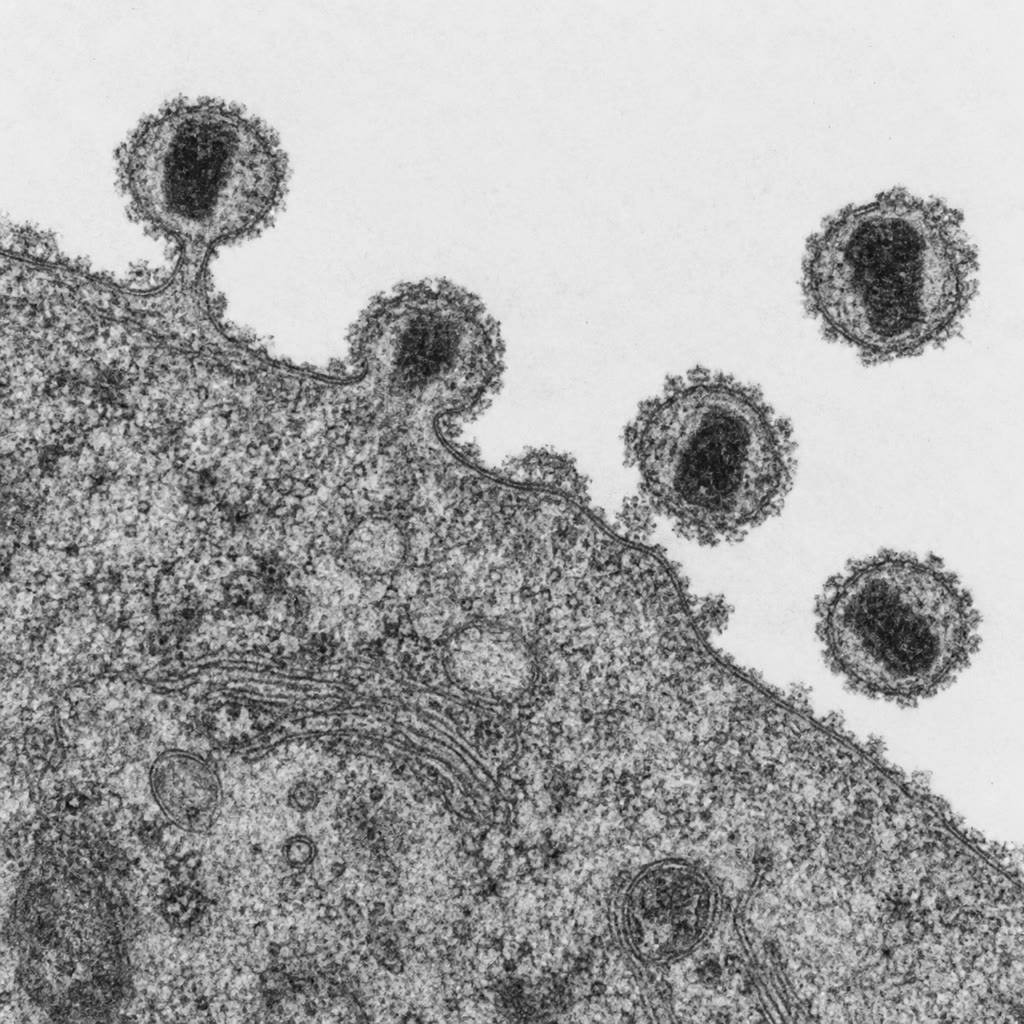
\includegraphics[width=0.36\linewidth]{images/book5/ai/b5-13-hiv-budding.jpg}

{\small Kiri: plak di dalam sebuah hamparan bakteri, masing-masing sebuah zona
bening tempat keturunan satu fag telah melisiskan sel di sekitarnya. Kanan:
partikel HIV yang menguncup dari sebuah limfosit~T, yang mengambil \omterm{def:b3:virology:virus}{selubungnya}
dari membran sel itu.}
\end{omfigure}

\begin{theorem}[Dinamika infeksi di dalam satu inang]\label{thm:b3:virology:dynamics}
\index{bilangan reproduksi dasar!dalam-inang}\index{muatan virus}%
\index{dinamika virus}
Misalkanlah $T$ kerapatan sel sasaran yang rentan, $I$ kerapatan sel yang
terinfeksi, dan $V$ kerapatan \omterm{def:b3:virology:virus}{virion} bebas. \omterm{def:b3:virology:virus}{Virion} menginfeksi sasaran dengan
laju $\beta TV$, sel terinfeksi menghasilkan \omterm{def:b3:virology:virus}{virion} dengan laju $p$ tiap sel
lalu mati dengan laju $\delta$, dan \omterm{def:b3:virology:virus}{virion} bebas disingkirkan dengan laju $c$:
\[
\frac{\mathrm{d}I}{\mathrm{d}t} = \beta TV - \delta I, \qquad
\frac{\mathrm{d}V}{\mathrm{d}t} = pI - cV .
\]
Dengan $T$ ditahan tetap, infeksinya tumbuh bila \emph{bilangan reproduksi
dasar} $R_{0} = \beta Tp/(c\delta)$ melebihi $1$, dan pada keadaan mantap
$V^{*} = p I^{*}/c$ dengan produksi mengimbangi penyingkiran.
Bila sebuah obat menghentikan semua infeksi baru pada $t = 0$ ($\beta \to 0$),
\omterm{def:b3:virology:virus}{virion} meluruh mula-mula dengan laju penyingkiran $c$, lalu, begitu \omterm{def:b3:virology:virus}{virus} bebas
turun ke aras yang dipertahankan sel terinfeksi yang tersisa, dengan laju
kematian $\delta$ sel itu:
\[
V(t) \approx V_{0}\,\frac{c\,e^{-\delta t} - \delta\,e^{-ct}}{c - \delta}
\;\longrightarrow\; V_{0}\,\frac{c}{c-\delta}\,e^{-\delta t}
\quad (t \gg 1/c).
\]
Kedua kemiringan \omterm{thm:b3:virology:dynamics}{muatan virus} sesudah pengobatan mengukur $c$ dan
$\delta$, dan $pI^{*} = cV^{*}$ memberikan produksi \omterm{def:b3:virology:virus}{virion} harian
sebelum pengobatan.
\end{theorem}
\begin{proof}
Sebuah sel terinfeksi hidup rata-rata $1/\delta$ dan membuat $p/\delta$
\omterm{def:b3:virology:virus}{virion}; tiap \omterm{def:b3:virology:virus}{virion} hidup $1/c$ lalu menginfeksi $\beta T/c$ sel dalam waktu
itu; hasil kalinya adalah banyaknya sel terinfeksi yang ditimbulkan satu sel
terinfeksi, yaitu $R_{0}$. Pada keadaan mantap $\mathrm{d}V/\mathrm{d}t = 0$
memberikan $V^{*} = pI^{*}/c$. Sesudah pengobatan $\mathrm{d}I/\mathrm{d}t =
-\delta I$, sehingga $I = I_{0}e^{-\delta t}$, dan $\mathrm{d}V/\mathrm{d}t =
pI_{0}e^{-\delta t} - cV$ adalah persamaan linear yang penyelesaiannya dengan
$V(0) = V_{0} = pI_{0}/c$ berupa ungkapan yang diberikan (periksalah: pada
$t = 0$ ia sama dengan $V_{0}$, dan ia memenuhi persamaannya suku demi suku).
Bagi $t
\gg 1/c$ suku $e^{-ct}$ telah lenyap dan $V$ mengikuti sel terinfeksi
dengan kemiringan $-\delta$; bagi $t \ll 1/\delta$ dan $c \gg \delta$
kemiringan awalnya $-c$.
\end{proof}

\begin{example}[HIV sebelum dan sesudah persamaannya]\label{ex:b3:virology:hiv}
Sampai tahun 1995 tahun-tahun \omterm{def:b3:virology:cycle}{latensi} klinis infeksi HIV --- \omterm{thm:b3:virology:dynamics}{muatan virus} yang
mantap sebesar $10^{4}$--$10^{6}$ salinan per mililiter dan penurunan lambat
sel~T --- dibaca sebagai \omterm{def:b3:virology:virus}{virus} yang lelap. Ho, Perelson, dan rekannya memberi
pasien sebuah \omterm{def:b3:virology:drugs}{penghambat protease} lalu mencocokkan penurunan \omterm{thm:b3:virology:dynamics}{muatan virus} itu
dengan teoremanya: fase cepatnya memberi $c \approx \qty{3}{d^{-1}}$
(paruh hidup \omterm{def:b3:virology:virus}{virion} sekitar enam jam), fase lambatnya $\delta \approx
\qty{0.5}{d^{-1}}$ (sebuah sel terinfeksi hidup sekitar satu setengah hari).
Muatan mantap sebesar $10^{5}$ per mililiter di dalam \qty{15}{L} cairan tubuh,
yang disingkirkan dengan laju $c$, karena itu menuntut produksi sekitar
$10^{10}$ \omterm{def:b3:virology:virus}{virion} sehari, tiap hari, bertahun-tahun: masa ``laten'' itu adalah
keadaan mantap infeksi dan kematian yang garang, dengan kumpulan sel~T
tergantikan tiap hari sampai ia gagal. Aritmetika mutasi pada bagian berikutnya
lalu menyusul seketika, dan bersamanya alasan mengapa obat tunggal gagal
sementara tiga obat tidak.
\end{example}

\begin{omfigure}
\begin{tikzpicture}
\begin{axis}[
  width=0.7\linewidth, height=5.8cm,
  axis x line=bottom, axis y line=left,
  xmin=0, xmax=14, ymin=10, ymax=2e5, ymode=log,
  xlabel={hari sesudah terapi dimulai}, ylabel={virion per mL},
  xlabel style={font=\small, at={(axis description cs:0.5,-0.12)}, anchor=north}, ylabel style={font=\small},
  tick label style={font=\small}, xtick={0,2,4,6,8,10,12,14},
  clip=false,
]
\addplot[very thick, omDef, domain=0:14, samples=100] {1e5*(3*exp(-0.5*x) - 0.5*exp(-3*x))/2.5};
\addplot[dashed, omThm, domain=0:1.6, samples=2] {1e5*exp(-3*x)};
\addplot[dashed, omMeth!70!black, domain=1.5:14, samples=2] {1e5*1.2*exp(-0.5*x)};
\node[font=\scriptsize, omThm, anchor=west] at (axis cs:1.8,600) {virion bebas disingkirkan: kemiringan $-c$, paruh hidup \qty{6}{h}};
\node[font=\scriptsize, omMeth!70!black, anchor=south west] at (axis cs:5.5,1.5e4) {sel terinfeksi mati: kemiringan $-\delta$, paruh hidup \qty{1.4}{d}};
\end{axis}
\end{tikzpicture}

{\small \omterm{thm:b3:virology:dynamics}{Muatan virus} sesudah sebuah obat menghentikan infeksi baru, dari
teoremanya dengan $c = \qty{3}{d^{-1}}$ dan $\delta = \qty{0.5}{d^{-1}}$:
sebuah penurunan cepat sementara \omterm{def:b3:virology:virus}{virion} bebas disingkirkan, lalu penurunan yang
lebih lambat yang dilangkahi kematian sel yang sudah terinfeksi.}
\end{omfigure}

\section{Bagaimana virus berevolusi}

\begin{definition}[Mutasi, kuasispesies, hanyutan dan pergeseran]\label{def:b3:virology:evolution}
\index{kuasispesies}\index{hanyutan antigen}%
\index{pergeseran antigen}\index{penyusunan ulang}
Polimerase bergantung-RNA dan transkriptase balik tidak melakukan \omterm{prop:b3:dna-repair:fidelity}{uji baca},
dan \omterm{def:b3:virology:virus}{virus} RNA bermutasi pada $10^{-4}$ sampai $10^{-6}$ per nukleotida per
penggandaan --- seribu sampai sejuta kali laju inangnya --- sehingga sebuah
populasi \omterm{def:b3:virology:virus}{virus} RNA berupa awan genom berkerabat, sebuah \emph{kuasispesies},
yang di dalamnya tiap mutan titik tunggal hadir setiap saat bila populasinya
besar. Seleksi oleh antibodi mendorong \emph{hanyutan antigen}: protein
permukaan influenza menimbun substitusi tahun demi tahun, dan imunitas tahun
lalu makin sedikit melindungi tiap musim. \emph{Pergeseran antigen} adalah
sebuah lompatan: sebuah genom bersegmen (influenza punya delapan segmen RNA)
dapat \emph{disusun ulang} ketika dua galur menginfeksi satu sel, dan sebuah
segmen yang menyandi sebuah hemaglutinin dari \omterm{def:b3:virology:virus}{virus} burung atau babi, yang
terhadapnya tidak seorang manusia pun punya imunitas, menghasilkan sebuah
pandemi --- 1918, 1957, 1968, 2009. Rekombinasi di dalam sebuah genom melakukan
hal yang sama bagi \omterm{def:b3:virology:virus}{virus} yang tidak bersegmen, dan koronavirus berekombinasi
dengan leluasa. Kebanyakan \omterm{def:b3:virology:virus}{virus} manusia yang baru adalah \emph{zoonosis}, yang
menyeberang dari sebuah wadah hewan --- kelelawar bagi koronavirus, Ebola, dan
rabies; burung dan babi bagi influenza; primata bagi HIV --- dan penyeberangan
itu biasanya soal beberapa mutasi pada sebuah protein pengikat reseptor.
\end{definition}

\begin{proposition}[Ambang galat]\label{prop:b3:virology:error-threshold}
\index{ambang galat}\index{uji baca!virus}
Sebuah genom beranggota $L$ nukleotida yang disalin dengan laju galat $u$ per
nukleotida tersalin tanpa galat sama sekali dengan peluang
$(1-u)^{L} \approx e^{-uL}$. Agar urutan yang terbugar bertahan di dalam
populasinya melawan banjir mutannya, pecahan salinan yang bebas galat harus
melebihi kira-kira kebalikan keunggulan terpilihnya $\sigma$: $e^{-uL} \gtrsim
1/\sigma$, yakni $uL \lesssim \ln\sigma$, sebuah bilangan berorde satu. Hasil
kali laju mutasi dan panjang genom karena itu terbatas: sebuah \omterm{def:b3:virology:virus}{virus} RNA
dengan $u = 10^{-4}$ tidak dapat memiliki genom yang jauh lebih panjang
daripada $10^{4}$ nukleotida, yang kira-kira sepanjang genom \omterm{def:b3:virology:virus}{virus} RNA, dan
koronavirus, yang pada \qty{30}{kb} merupakan genom RNA terpanjang yang
dikenal, mencapainya hanya dengan menyandi sebuah eksonuklease penguji baca
yang memangkas $u$ sepuluh kali lipat. Ambangnya juga sebuah senjata: obat yang
menaikkan laju galat polimerase (ribavirin, molnupiravir) mendorong sebuah
\omterm{def:b3:virology:virus}{virus} melewatinya masuk ke \emph{bencana galat}, dan \omterm{def:b3:virology:evolution}{kuasispesiesnya} runtuh.
\end{proposition}
\begin{proof}
Galat yang saling bebas pada tiap dari $L$ tapak memberikan peluang bebas galat
$(1-u)^{L}$, dan $\ln(1-u) \approx -u$ bagi $u$ yang kecil. Neraca
populasinya adalah hujah \omterm{def:b3:virology:evolution}{kuasispesies} yang baku (Eigen, 1971): urutan induknya
diisi ulang dengan laju $\sigma e^{-uL}$ relatif terhadap mutan rata-rata
lalu hilang karena mutasi selebihnya; ia dipertahankan hanya bila yang
pertama melebihi $1$, dan dari situlah batas itu berasal.
\end{proof}

\begin{omfigure}
\begin{tikzpicture}[every node/.style={font=\scriptsize}, >=stealth]
  % drift
  \begin{scope}
    \foreach \i in {0,1,2,3} { \draw[thick, omProp, fill=omProp!30] (\i*1.3,0) circle (0.35); \foreach \a in {0,60,...,300} \draw[omProp, thick] (\i*1.3,0) ++(\a:0.35) -- ++(\a:0.14); }
    \foreach \i/\n in {1/1,2/2,3/3} { \foreach \k in {1,...,\n} \fill[omThm] (\i*1.3,0) ++({60*\k+20}:0.5) circle (0.06); }
    \foreach \i in {0,1,2} \draw[->, thick] (\i*1.3+0.5,0) -- (\i*1.3+0.8,0);
    \node[below, align=center] at (1.95,-0.6) {hanyutan antigen: mutasi titik menimbun\\di protein permukaan, musim demi musim};
  \end{scope}
  % shift
  \begin{scope}[xshift=7.0cm]
    \draw[thick, omProp, fill=omProp!30] (0,0.5) circle (0.4); \foreach \y in {-0.2,-0.1,0,0.1,0.2} \draw[omProp!80!black] (-0.25,0.5+\y) -- (0.25,0.5+\y);
    \draw[thick, omMeth!70!black, fill=omMeth!30] (0,-0.7) circle (0.4); \foreach \y in {-0.2,-0.1,0,0.1,0.2} \draw[omMeth!70!black] (-0.25,-0.7+\y) -- (0.25,-0.7+\y);
    \node[left, align=right] at (-0.5,0.5) {galur manusia,\\8 segmen}; \node[left, align=right] at (-0.5,-0.7) {galur burung,\\8 segmen};
    \draw[->, thick] (0.5,0.4) -- (1.5,0.0); \draw[->, thick] (0.5,-0.6) -- (1.5,-0.2);
    \draw[thick, omDef, fill=omDef!10] (2.4,-0.1) ellipse (0.9 and 0.7); \node[below] at (2.4,-0.85) {satu sel (seekor babi)};
    \draw[->, thick] (3.4,-0.1) -- (4.3,-0.1);
    \draw[thick, omProp, fill=omProp!30] (4.9,-0.1) circle (0.4); \foreach \y in {-0.2,-0.1,0.1,0.2} \draw[omProp!80!black] (4.65,-0.1+\y) -- (5.15,-0.1+\y); \draw[omMeth!70!black, very thick] (4.65,-0.1) -- (5.15,-0.1);
    \node[right, align=left] at (5.4,-0.1) {penyusunan ulang:\\hemaglutinin burung\\di virus manusia};
    \node[below, align=center] at (2.4,-1.5) {pergeseran antigen: segmen utuh dipertukarkan;\\tak seorang pun kebal --- sebuah pandemi};
  \end{scope}
\end{tikzpicture}

{\small Dua cara sebuah \omterm{def:b3:virology:virus}{virus} influenza lolos dari imunitas. Hanyutan: mutasi
pada durinya menimbun secara berangsur. Pergeseran: dua galur di dalam satu sel
menukar segmen genom utuh, dan sebuah protein duri yang baru bagi manusia
muncul sekaligus.}
\end{omfigure}

\begin{example}[Mengapa HIV memerlukan tiga obat]\label{ex:b3:virology:three-drugs}
Transkriptase balik HIV keliru sekitar sekali tiap $10^{5}$ nukleotida,
sehingga tiap genom \qty{9700}{nt} yang disalin mengusung sekitar $0.1$ mutasi,
dan $10^{10}$ genom baru sehari mengusung $10^{9}$ mutasi di antaranya: tiap
satu dari $3\times 9700 \approx \num{30000}$ mutasi titik tunggal yang mungkin
muncul berkali-kali setiap hari, sebelum obat apa pun diberikan. Sebuah obat
yang dikalahkan satu mutasi --- sebagaimana satu mutasi mengalahkan kebanyakan
penghambat transkriptase balik dan \omterm{def:b3:virology:drugs}{penghambat protease} --- karena itu
dikalahkan dalam hitungan minggu, dan itulah yang menimpa AZT pada tahun 1987.
Dua mutasi yang saling bebas muncul bersama pada $10^{-10}$ per genom, sekitar
sekali sehari; tiga mutasi pada $10^{-15}$, sekali tiap seribu hari --- dan
seorang pasien dengan tiga obat yang muatannya telah turun seribu kali lipat
menghasilkan $10^{7}$ genom sehari, sehingga mutan rangkap tiga itu tidak
pernah muncul. Hal itu, dan pembuktian teoremanya bahwa \omterm{def:b3:virology:virus}{virusnya} sedang
menggandakan diri dengan kecepatan penuh, menjadikan \omterm{thm:b3:cancer-biology:goldie-coldman}{terapi gabungan} sejak
tahun 1996 pengobatan yang mengubah AIDS menjadi sebuah keadaan menahun.
\end{example}

\section{Inang, pertahanan, dan obat}

\begin{proposition}[Patogenesis dan pertahanan]\label{prop:b3:virology:pathogenesis}
\index{efek sitopatik}\index{interferon}\index{restriksi!fag}
Sebuah \omterm{def:b3:virology:virus}{virus} merugikan dengan melisiskan sel (polio memusnahkan neuron motorik,
HIV membunuh sel~T), dengan membuat sel menghasilkan produk beracun, dengan
mengubahnya (\cref{ch:b3:cancer-biology}), dan kerap terutama lewat tanggapan
inang itu sendiri: demam, kerusakan jaringan dan, pada keadaan terburuk, badai
sitokin reaksi imun terhadap influenza atau koronavirus SARS. Inangnya
menjawab dengan pertahanan bawaan yang mengenali tanda tangan penggandaan
\omterm{def:b3:virology:virus}{virus} --- RNA untai ganda, RNA tanpa tudung, DNA di dalam sitosol --- lalu
menanggapinya dengan \emph{interferon}, yang menaruh tiap sel tetangga ke dalam
keadaan antivirus (\cref{ch:b3:innate-immunity}); dengan sel pembunuh alami
yang memusnahkan sel yang telah menyembunyikan MHC-nya; dengan antibodi yang
menetralkan \omterm{def:b3:virology:virus}{virion} dan sel~T sitotoksik yang membunuh sel terinfeksi sebelum
sel itu melepaskan keturunannya (\cref{ch:b3:adaptive-immunity});
dan, pada bakteri, dengan \omterm{def:b3:genetic-engineering:tools}{enzim restriksi} yang memotong DNA asing serta ingatan
\omterm{def:b3:genetic-engineering:crispr}{CRISPR} pada \cref{ch:b3:genetic-engineering}. \omterm{def:b3:virology:virus}{Virus} menjawab balik: hampir tiap
\omterm{def:b3:virology:virus}{virus} besar menyandi protein yang menghalangi interferon, menyembunyikan MHC,
meniru sitokin, atau menghambat \omterm{def:b3:cell-cycle-apoptosis:apoptosis}{apoptosis}, dan perlombaan senjatanya tertulis
di dalam kedua genom.
\end{proposition}

\begin{definition}[Obat antivirus dan vaksin]\label{def:b3:virology:drugs}
\index{obat antivirus}\index{analog nukleosida}\index{penghambat protease}%
\index{vaksin}\index{vaksin mRNA}
Obat antivirus menyerang enzim \omterm{def:b3:virology:virus}{virus} atau langkah yang tidak dilakukan sel
inang. \emph{Analog nukleosida} adalah penamat rantai: asiklovir
difosforilasi hanya oleh timidin kinase herpesvirus lalu menghalangi DNA
polimerase \omterm{def:b3:virology:virus}{virus}, sehingga ia bekerja hanya di dalam sel terinfeksi;
AZT, tenofovir, dan lamivudin menghentikan transkriptase balik; remdesivir dan
molnupiravir bekerja pada polimerase koronavirus, yang kedua lewat
mutagenesis. \emph{Penghambat protease} menghalangi pemotongan poliprotein
\omterm{def:b3:virology:virus}{virus} (HIV, hepatitis C, nirmatrelvir bagi SARS-CoV-2). Penghambat integrase
menghentikan pembentukan provirus HIV; penghambat neuraminidase menghentikan
\omterm{def:b3:virology:virus}{virion} influenza melepaskan diri dari sel yang darinya ia menguncup; penghambat
pemasukan menghalangi sebuah reseptor. \omterm{def:b3:virology:virus}{Virus} hepatitis C kini disembuhkan dalam
dua belas minggu oleh gabungan obat yang bekerja langsung, yakni infeksi \omterm{def:b3:virology:virus}{virus}
menahun pertama yang pernah disembuhkan oleh kemoterapi. \emph{Vaksin}
menyajikan antigen \omterm{def:b3:virology:virus}{virus} tanpa penyakitnya: sebuah \omterm{def:b3:virology:virus}{virus} hidup yang dilemahkan
(campak, polio lewat mulut, demam kuning), sebuah \omterm{def:b3:virology:virus}{virus} yang dimatikan (polio
lewat suntikan, influenza), sebuah subunit (antigen permukaan hepatitis B yang
dibuat di dalam khamir, protein \omterm{def:b3:virology:virus}{kapsid} \omterm{def:b3:virology:virus}{virus} papiloma), sebuah vektor \omterm{def:b3:virology:virus}{virus} tak
berbahaya yang mengusung sebuah gen sasarannya, atau, sejak tahun 2020,
\emph{RNA duta} yang menyandi antigennya, yang diantarkan di dalam nanopartikel
lipid, yang diterjemahkan oleh sel penerimanya sendiri. Imunologi mengapa
semuanya bekerja, dan berapa banyak orang yang harus divaksinasi untuk
melindungi sisanya, adalah pokok \cref{ch:b3:adaptive-immunity}.
\end{definition}

\begin{remark}[Virus dalam ekonomi kehidupan]\label{rem:b3:virology:economy}
\omterm{def:b3:virology:virus}{Virus} yang merugikan manusia hanyalah galat pembulatan di dalam populasi \omterm{def:b3:virology:virus}{virus}
dunia, yang kebanyakannya menginfeksi bakteri dan arkea. Fag membunuh
seperlima sampai sepertiga bakteri lautan tiap hari lalu mengembalikan isinya
ke kumpulan terlarut --- \emph{pintasan \omterm{def:b3:virology:virus}{virus}} pada daur karbon di dalam jilid
Tahun~2. Mereka memindahkan gen antarbakteri
(\cref{ch:b3:bacteriology}), dan racunnya adalah racun
difteri, kolera, dan \emph{E.~coli} yang terburuk. Delapan persen genom
manusia adalah sisa retrovirus purba
(\cref{ch:b3:genomics}), yang salah satu gen \omterm{def:b3:virology:virus}{selubungnya} kini meleburkan
sel plasenta. \omterm{def:b3:virology:virus}{Virus} adalah wadah kebaruan genetik terbesar
di planet ini, dan batas antara apa yang terhitung hidup melintas
di tengah mereka.
\end{remark}

\section{Latihan}

\begin{exercise}[$\star$]\label{exo:b3:virology:1}
Tempatkanlah polio, influenza, HIV, herpes simpleks, hepatitis B, dan rotavirus
pada kelas Baltimore-nya lalu sebutkanlah enzim apa yang harus dibawa atau
dibuat masing-masing yang tidak dipunyai sel.
\end{exercise}

\begin{exercise}[$\star$]\label{exo:b3:virology:2}
Apa yang ditunjukkan percobaan Hershey--Chase, dan apa yang akan ditemukan
seandainya proteinlah yang mengusung petunjuknya?
\end{exercise}

\begin{exercise}[$\star$]\label{exo:b3:virology:3}
Sebuah stok fag yang diencerkan $10^{-7}$ memberi $84$ plak dari \qty{0.1}{mL}.
Berapa titernya? Mengapa mikroskop elektron dapat mencacah partikel sepuluh
kali lebih banyak?
\end{exercise}

\begin{exercise}[$\star$]\label{exo:b3:virology:4}
Sebutkanlah keenam tahap sebuah daur replikasi dan, bagi tiap tahap, namailah
satu \omterm{def:b3:virology:drugs}{obat antivirus} atau satu pertahanan inang yang bekerja padanya.
\end{exercise}

\begin{exercise}[$\star\star$]\label{exo:b3:virology:5}
Dengan memakai \cref{prop:b3:virology:economy}, hitunglah asam nukleat yang
diperlukan untuk menyandi \omterm{def:b3:virology:virus}{kapsid} sebuah \omterm{def:b3:virology:virus}{virus} yang terbuat dari $180$ salinan
sebuah protein \qty{30}{kDa}, lalu bandingkanlah dengan genom \qty{4.5}{kb}
yang mungkin dipunyai \omterm{def:b3:virology:virus}{virus} semacam itu. Berapa pecahan genom yang berupa gen
\omterm{def:b3:virology:virus}{kapsidnya}?
\end{exercise}

\begin{exercise}[$\star\star$]\label{exo:b3:virology:6}
Dengan $c = \qty{3}{d^{-1}}$, $\delta = \qty{0.5}{d^{-1}}$, dan $V_{0} =
10^{5}$ per mL, hitunglah $V$ dari teoremanya pada $t = 0.5$, $2$, dan
$10$ hari. Berapa lama sampai muatannya turun di bawah $50$ per mL, yakni batas
pendeteksian?
\end{exercise}

\begin{exercise}[$\star\star$]\label{exo:b3:virology:7}
Sebuah \omterm{def:b3:virology:virus}{virus} RNA memiliki $u = 3\times 10^{-5}$ dan $L = \qty{12}{kb}$. Berapa
pecahan genom keturunannya yang tidak mengusung mutasi? Apa yang terjadi pada
pecahan itu bila sebuah obat mutagen menaikkan $u$ tiga kali lipat? Jelaskanlah
mengapa koronavirus memerlukan sebuah enzim penguji baca.
\end{exercise}

\begin{exercise}[$\star\star$]\label{exo:b3:virology:8}
Jelaskanlah hanyutan dan \omterm{def:b3:virology:evolution}{pergeseran antigen} pada influenza, dan mengapa sebuah
galur pandemi sejauh ini selalu mengusung sebuah hemaglutinin baru.
\end{exercise}

\begin{exercise}[$\star\star$]\label{exo:b3:virology:9}
Asiklovir adalah sebuah analog guanosin yang harus difosforilasi agar bekerja.
Jelaskanlah mengapa ia merugikan sel yang terinfeksi herpes dan bukan sel lain,
lalu ramalkanlah mutasi kekebalannya.
\end{exercise}

\begin{exercise}[$\star\star\star$]\label{exo:b3:virology:10}
Turunkanlah $R_{0} = \beta Tp/(c\delta)$ dari kedua persamaan teoremanya dengan
mencari syarat agar sebuah infeksi kecil ($I$, $V$ dekat nol, $T$ tetap)
bertumbuh, lalu tafsirkanlah tiap faktornya.
\end{exercise}

\begin{exercise}[$\star\star\star$]\label{exo:b3:virology:11}
Seorang pasien dengan terapi yang mujarab masih menyimpan $10^{6}$ sel~T
beristirahat yang terinfeksi laten dan provirusnya bungkam, dengan paruh hidup
$44$ bulan. Berapa lama terapinya harus berlanjut agar wadah itu turun di bawah
satu sel? Mengapa hal ini membuat HIV tidak tersembuhkan oleh obat yang
menghalangi penggandaan, dan apa yang akan dituntut sebuah kesembuhan?
\end{exercise}

\begin{exercise}[$\star\star\star$]\label{exo:b3:virology:12}
Jelaskanlah hujah \cref{ex:b3:virology:three-drugs} dengan angka Anda sendiri
bagi sebuah \omterm{def:b3:virology:virus}{virus} \qty{30}{kb} dengan $u = 10^{-6}$ yang menghasilkan $10^{9}$
genom sehari. Berapa banyak obat yang akan Anda gabungkan, dan mengapa obat
terhadap dua tapak enzim yang sama mungkin tidak terhitung dua?
\end{exercise}

\section{Soal: Sebuah Virus di dalam Seorang Pasien}

\begin{problem}[{Soal akhir pekan --- sebuah infeksi HIV yang dicacah virion
demi virion, dinamikanya dicocokkan dengan sebuah kurva pengobatan, mutasinya
dihitung terhadap obatnya, dan wadahnya ditakar waktunya, berakhir pada
produksi virion harian, hari ketika muatannya menjadi tak terdeteksi, serta
peluang bahwa sebuah mutan rangkap tiga ada}]
\label{pb:b3:virology:1}
Data: \omterm{thm:b3:virology:dynamics}{muatan virus} $V^{*} = 2\times 10^{5}$ per mL di dalam \qty{15}{L} cairan
tubuh; $c = \qty{3}{d^{-1}}$, $\delta = \qty{0.5}{d^{-1}}$; tiap sel terinfeksi
membuat $p = 500$ \omterm{def:b3:virology:virus}{virion} sehari; genom \qty{9700}{nt}, $u = 10^{-5}$
per nukleotida per penggandaan; mutasi tunggal memberi kekebalan terhadap
masing-masing dari tiga obat; pada terapi rangkap tiga produksinya turun ke
$10^{7}$ genom sehari; wadah laten $10^{6}$ sel, paruh hidup $44$ bulan;
sebuah \omterm{def:b3:virology:virus}{virion} berupa bola \qty{120}{nm} yang berisi dua untai RNA \qty{9700}{nt}
dan sekitar \num{2000} molekul protein \qty{25}{kDa}.

\medskip
\noindent\textbf{Bagian I --- Mencacah.}
\begin{enumerate}
  \item Berapa banyak \omterm{def:b3:virology:virus}{virion} yang ada di dalam tubuh pada keadaan mantap?
  \item Berapa banyak yang disingkirkan tiap hari, dan karenanya dihasilkan
        tiap hari?
  \item Berapa banyak sel terinfeksi yang menghasilkannya, dan berapa banyak
        yang mati tiap hari?
  \item Berapa massa satu \omterm{def:b3:virology:virus}{virion} (RNA sebesar \qty{330}{Da} per
        nukleotida ditambah proteinnya), dan berapa massa total \omterm{def:b3:virology:virus}{virion} di dalam
        tubuh? Bandingkanlah dengan sebutir pasir (\qty{1}{mg}).
  \item Tubuh punya $10^{12}$ sel~T CD4 dan menggantikan yang
        terinfeksi. Berapa pecahan kumpulan itu yang terinfeksi setiap saat,
        dan bagaimana pecahan sekecil itu membunuh kumpulannya dalam sepuluh
        tahun?
  \item Bila tiap sel terinfeksi mati dengan \omterm{def:b3:cell-cycle-apoptosis:apoptosis}{apoptosis} lalu ditelan dalam
        sejam (\cref{ch:b3:cell-cycle-apoptosis}), berapa banyak yang sedang
        disingkirkan setiap saat?
\end{enumerate}

\medskip
\noindent\textbf{Bagian II --- Pengobatan.}
\begin{enumerate}[resume]
  \item Terapi menghentikan infeksi baru pada $t = 0$. Hitunglah $V$ pada $t =
        1$, $3$, $7$, dan $14$ hari dari teoremanya.
  \item Pada hari keberapa muatannya turun di bawah batas pendeteksian
        $50$ per mL?
  \item Dari kedua kemiringan, bagaimana seorang klinisi akan menaksir $c$ dan
        $\delta$ dari pengukuran pada hari $0$--$1$ dan $3$--$10$?
  \item Sesudah kedua fase itu muatannya mendatar pada beberapa salinan per mL
        lalu bertahan di sana bertahun-tahun. Petak model mana yang hilang,
        dan berapa laju peluruhannya?
  \item Hitunglah paruh hidup sebuah \omterm{def:b3:virology:virus}{virion} bebas dan sebuah sel terinfeksi.
  \item Jelaskanlah mengapa dataran sebelum pengobatan salah dibaca sebagai
        \omterm{def:b3:virology:cycle}{latensi}, dan apa yang justru ditunjukkan persamaannya.
\end{enumerate}

\medskip
\noindent\textbf{Bagian III --- Mutasi.}
\begin{enumerate}[resume]
  \item Mutasi per genom per penggandaan, dan mutasi yang dihasilkan
        tiap hari pada pasien yang tidak diobati.
  \item Berapa banyak mutasi titik tunggal berbeda yang mungkin di dalam
        genomnya? Berapa kali tiap hari masing-masing muncul?
  \item Laju per genom sebuah mutan rangkap dua tertentu dan sebuah mutan
        rangkap tiga tertentu; berapa banyak masing-masing muncul tiap hari
        tanpa obat?
  \item Pada terapi rangkap tiga, dengan $10^{7}$ genom sehari, berapa harapan
        mutan rangkap tiga tiap tahun?
  \item Pasiennya melewatkan dosis sehingga aras satu obat jatuh ke
        nol selama seminggu sementara kedua obat lain bertahan. Mutan mana yang
        kini dapat terpilih, dan berapa harapan banyaknya
        mutan rangkap dua yang bersangkutan yang dihasilkan pada minggu itu
        pada $10^{7}$ genom sehari?
  \item Mengapa kekebalan terhadap satu \omterm{def:b3:virology:drugs}{analog nukleosida} kerap memberi
        kekebalan terhadap analog lain, dan bagaimana hal itu mengubah cacah
        obat yang ``saling bebas''?
\end{enumerate}

\medskip
\noindent\textbf{Bagian IV --- Wadah dan kesembuhan.}
\begin{enumerate}[resume]
  \item Dengan paruh hidup $44$ bulan, berapa lama sampai $10^{6}$
        sel laten turun menjadi satu? Menjadi $10^{4}$?
  \item Bila terapinya dihentikan, satu sel laten yang mengaktif kembali sudah
        cukup untuk memulai lagi infeksinya. Berapa lama sesudah dihentikan
        muatannya kembali ke $10^{5}$ per mL, bila ia tumbuh dengan
        $R_{0} = 8$ per generasi $2$ hari dari satu \omterm{def:b3:virology:virus}{virion}?
  \item Usulkanlah dua siasat kesembuhan yang menyusul dari modelnya,
        lalu nyatakanlah penghalang bagi masing-masing.
  \item $R_{0}$ teoremanya berlaku di dalam satu inang. Sebuah $R_{0}$
        populasi bagi HIV antarorang sekitar $3$--$5$. Berapa pecahan
        penularan yang harus dicegah untuk mengakhiri wabahnya
        ($1 - 1/R_{0}$)?
  \item Pengobatan menurunkan kemampuan menular seorang pasien pada dasarnya
        ke nol. Jelaskanlah bagaimana ``pengobatan sebagai pencegahan''
        menyusul dari teorema dalam-inang itu.
  \item Sebuah \omterm{def:b3:virology:drugs}{vaksin} berkemujaraban $E$ (pecahan orang tervaksinasi yang
        terlindungi) yang diberikan kepada pecahan $f$ populasi melindungi
        $Ef$ bagiannya. Cakupan $f$ berapa yang diperlukan untuk mencapai
        ambang pertanyaan sebelumnya dengan $E = 0.7$? Dengan $E = 0.9$? Apa
        makna jawaban yang pertama?
  \item Ringkaslah: \omterm{def:b3:virology:virus}{virion} yang dihasilkan tiap hari (pertanyaan~2), hari
        ketika muatannya menjadi tak terdeteksi (pertanyaan~8), serta harapan
        banyaknya mutan rangkap tiga tiap tahun pada terapi (pertanyaan~16).
\end{enumerate}
\end{problem}
